% Graphical abstract for the MDPI submission form (1100 x 560 px at 200 dpi).
% Build: pdflatex graphical-abstract && pdftoppm -r 200 -png -singlefile graphical-abstract graphical-abstract
\documentclass{article}
\usepackage[paperwidth=5.5in,paperheight=2.8in,margin=0pt]{geometry}
\usepackage[T1]{fontenc}
\usepackage{mathptmx}
\usepackage{tikz}
\usetikzlibrary{arrows.meta,positioning}
\pagestyle{empty}
\setlength{\parindent}{0pt}
\begin{document}
\noindent\resizebox{5.3in}{!}{%
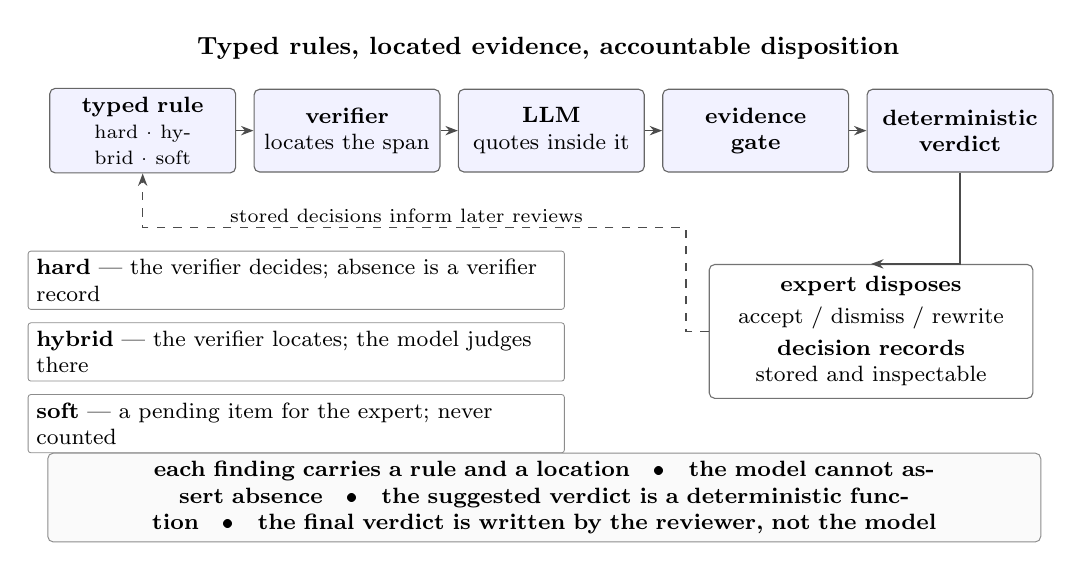
\begin{tikzpicture}[
  font=\sffamily,
  flow/.style={draw=black!60,rounded corners=2pt,line width=0.4pt,fill=blue!5,align=center,inner sep=3pt,text width=2.15cm,minimum height=1.05cm,font=\footnotesize},
  tier/.style={draw=black!45,rounded corners=1pt,line width=0.3pt,align=left,inner sep=3pt,text width=6.6cm,font=\footnotesize},
  arr/.style={-{Stealth[length=4.5pt]},line width=0.55pt,draw=black!70},
  fb/.style={-{Stealth[length=4.5pt]},line width=0.55pt,dashed,draw=black!70}
]
\node[font=\small\bfseries] at (6.8,6.5) {Typed rules, located evidence, accountable disposition};

\node[flow] (f1) at (1.65,5.45) {\textbf{typed rule}\\{\scriptsize hard · hybrid · soft}};
\node[flow,right=0.22cm of f1] (f2) {\textbf{verifier}\\locates the span};
\node[flow,right=0.22cm of f2] (f3) {\textbf{LLM}\\quotes inside it};
\node[flow,right=0.22cm of f3] (f4) {\textbf{evidence}\\\textbf{gate}};
\node[flow,right=0.22cm of f4] (f5) {\textbf{deterministic}\\\textbf{verdict}};
\draw[arr] (f1)--(f2); \draw[arr] (f2)--(f3); \draw[arr] (f3)--(f4); \draw[arr] (f4)--(f5);

\node[tier] (t1) at (3.6,3.55) {\textbf{hard} --- the verifier decides; absence is a verifier record};
\node[tier,below=0.16cm of t1.south,anchor=north] (t2) {\textbf{hybrid} --- the verifier locates; the model judges there};
\node[tier,below=0.16cm of t2.south,anchor=north] (t3) {\textbf{soft} --- a pending item for the expert; never counted};

\node[draw=black!55,rounded corners=2pt,line width=0.4pt,align=center,inner sep=3pt,text width=3.9cm,font=\footnotesize,minimum height=1.7cm] (exp) at (10.9,2.9) {\textbf{expert disposes}\\[2pt]accept / dismiss / rewrite\\[2pt]\textbf{decision records}\\stored and inspectable};

\draw[arr] (f5.south) |- (exp.north);
\draw[fb] (exp.west) -- (8.55,2.9) -- (8.55,4.22) -- (1.65,4.22) -- (f1.south);
\node[font=\scriptsize,anchor=south,fill=white,inner sep=1pt] at (5.0,4.24) {stored decisions inform later reviews};

\node[draw=black!45,rounded corners=2pt,line width=0.35pt,fill=black!2,align=center,text width=12.4cm,font=\footnotesize,inner sep=3pt,anchor=south] at (6.75,0.22) {\textbf{each finding carries a rule and a location}\quad\textbullet\quad\textbf{the model cannot assert absence}\quad\textbullet\quad\textbf{the suggested verdict is a deterministic function}\quad\textbullet\quad\textbf{the final verdict is written by the reviewer, not the model}};

\end{tikzpicture}}
\end{document}
